\chapter{Mapas caóticos}

    \section{Definición de caos}
    
        Una manera sencilla de definir el caos sin la necesidad de introducir conceptos muy complicados es como un comportamiento aperiódico, aparentemente impredecible, en sistemas deterministas los cuales presentan extrema sensibilidad a las condiciones iniciales, el más mínimo cambio en la condición inicial produce un resultado muy diferente. \cite{Strogatz1994}

        Según \cite{Sprott2003} los sistemas caóticos tienen las siguientes características:

        \begin{enumerate}
            \item Son aperiódicos, es decir nunca se repiten.
            \item Presentan una dependencia sensible de las condiciones iniciales (y, por tanto, son imprevisibles a largo plazo).
            \item Se rigen por uno o varios parámetros de control, una pequeña modificación de los cuales puede hacer aparecer o desaparecer el caos.
            \item Sus ecuaciones son no lineales.
        \end{enumerate}

        Los mapas caóticos, mapas iterados, ecuaciones de diferencias o simplemente mapas, son sistemas dinámicos en tiempo discreto que tienen la forma general $x_{n+1} = f(x_{n})$, los cuales requieren una condición inicial $x_{0}$ y se iteran continuamente para conocer su comportamiento. A la secuencia $x_{0}, x_{1}, x_{2} , \ldots $ se le conoce como la órbita del mapa comenzando desde $x_{0}$.

    \section{Puntos fijos y estabilidad lineal}

        Antes de comenzar a estudiar los mapas es necesario desarrollar algunas herramientas que nos sirvan para su análisis. Partimos de la ecuación general de los  $x_{n+1} = f(x_{n})$, supongamos que $x^{*}$ satisface que $f(x^{*}) = x^{*} $, entonces $x^{*}$ es un \emph{punto fijo}, si $x_{n} = x^{*} $ entonces $x_{n+1} = f(x_{n}) = x^{*} $, por lo tanto la órbita permanecerá en $x^{*} $ para todas las futuras iteraciones. 

        Para determinar la estabilidad de $x^{*}$, consideramos una órbita cercana $x_{n} = x^{*} + \eta_{n} $ y nos preguntamos si la órbita es atraída o repelida desde $x^{*}$. Es decir, ¿crece o decrece la desviación $\eta_{n}$ a medida que aumenta $n$?. Utilizando la expansión de Taylor y sustituyendo da como resultado:

        \begin{equation}
            x^{*} + \eta_{n+1} = x_{n+1} = f(x^{*} + \eta_{n}) = f(x^{*}) + f'(x^{*}) \eta_{n} + O(\eta_{n}^{2})
        \end{equation}

        Pero como $f(x^{*}) = x^{*} $, entonces la ecuación se reduce a:

        \begin{equation}
            \eta_{n+1} = f'(x^{*}) \eta_{n} + O(\eta_{n}^{2})
        \end{equation}

        Supongamos que podemos despreciar con seguridad los términos $O(\eta_{n}^{2} )$. Entonces obtenemos el mapa linealizado $ \eta_{n+1} = f'(x^{*}) \eta_{n}$ con multiplicador $\lambda = f'(x^{*} )$. La solución de este mapa linearizado puede hallarse explícitamente escribiendo unos pocos términos: $\eta_{1} = \lambda \eta_{0}$, $\eta_{2} = \lambda \eta_{1} = \lambda^{2} \eta_{0} $ y así en general $\eta_{n} = \lambda^{n} \eta_{0} $. Si $|\lambda| = |f'(x^{*})| < 1$, entonces $\eta_{n} \to 0$ a medida que $n \to \infty$ y el punto fijo $x^{*}$ es linealmente estable. Por el contrario, si $|f'(x^{*})| > 1$ el punto fijo es inestable. Aunque estas conclusiones sobre la estabilidad local se basan en la linealización, puede demostrarse que se mantienen para el mapa no lineal original. Pero la linealización no dice nada sobre el caso marginal $|f'(x^{*})| = 1$, entonces los términos $O(\eta_{n}^{2} )$ despreciados determinan la estabilidad local.

    \section{Mapa logístico}

        Cuando nos encontramos con un fenómeno complejo como el caos, que se manifiesta en diversas situaciones, es útil adoptar un enfoque que permita identificar y estudiar el sistema más simple que lo ejemplifica. En este sentido, el \emph{mapa logístico} representa el sistema matemático caótico más sencillo, ya que utiliza únicamente una variable y un parámetro de control. Las soluciones exactas de este sistema pueden obtenerse mediante álgebra y su representación gráfica facilita su visualización. Este modelo presenta muchas similitudes con sistemas caóticos más complejos, lo que lo convierte en un candidato perfecto para su estudio. De hecho, ha sido utilizado para modelar fenómenos en diversos campos como la ecología, oncología y finanzas.\cite{Sprott2003}

        La ecuación que define al mapa logístico se puede formular partiendo del modelo de crecimiento exponencial en tiempo discreto que se muestra en la ecuación (\ref{eq:crecimiento_exponencial}), donde $A$ es la tasa de crecimiento.

        \begin{equation}
            x_{n+1} = A x_{n}
            \label{eq:crecimiento_exponencial}
        \end{equation}

        Esta ecuación es un ejemplo de un sistema dinámico deterministas, en el que el valor siguiente de $x$ depende únicamente del valor actual. Se trata de un sistema lineal, ya que su representación gráfica muestra una línea recta al graficar $x_{n+1}$ contra $x_{n}$. Se trata de una relación recursiva, ya que se aplica de forma repetida a valores sucesivos de $n$. Además es un ejemplo de mapa iterado, iterar significa retroalimentar la salida de la ecuación a la entrada en el siguiente paso temporal mientas que la iteración es el valor resultante. El término mapa deriva del proceso de transferir cada punto de la Tierra a su correspondiente punto en un mapa impreso. En este caso, estamos mapeando un punto a lo largo del eje $x$ en otro punto a lo largo del mismo eje como se muestra en la Figura \ref{fig:F0_mapdiagram}. Sin embargo para mapas más complicados el mapeo se puede extender a más de una dimensión. 


        \begin{figure}[hbtp]
            \caption{Ejemplo de mapeo en una dimensión.}
            \centering
            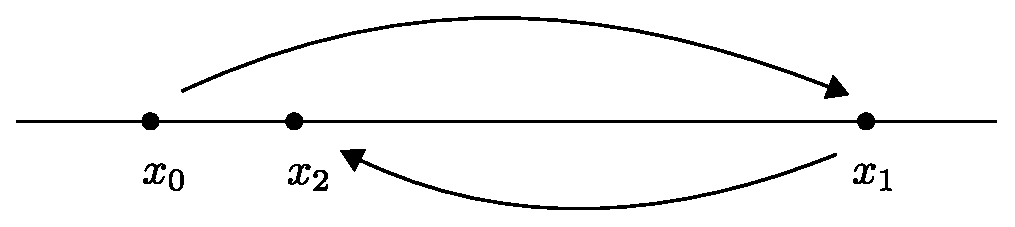
\includegraphics[width=0.7\textwidth]{F0_mapdiagram}
            \label{fig:F0_mapdiagram}
        \end{figure}


        Si el parámetro $A > 1$ el sistema presenta un crecimiento exponencial mientras que si $0 < A < 1$ presenta un decaimiento exponencial. Para toda condición inicial $x_{0}$ el sistema es atraído al punto $x = 0$ si $0 < A < 1$ y es atraído hacia el infinito si $A > 1$. Los sistemas cuya solución es atraída hacia el infinito son conocidos como no acotado. El termino $A$ es un parámetro de control que rige la naturaleza de la dinámica. El valor $A = 1$ separa dos regiones en las que el comportamiento difiere y se denomina punto de bifurcación. Si $|A| < 1$ el sistema oscila alrededor de $x = 0$ y su amplitud decrece con el tiempo. Por lo tanto $x = 0$ es un atractor para toda $x_{0}$ cuando $|A| < 1$. Sin embargo cuando $A< -1$ crece exponencialmente hacia el menos infinito.

        Como el crecimiento exponencial no puede continuar para siempre, la ecuación (\ref{eq:crecimiento_exponencial}) es poco realista para cualquier proceso natural. Típicamente, alguna no linealidad detiene e incluso revierte el crecimiento. La no linealidad es despreciable en pequeños valores de $x$ pero empieza a dominar mientras más crece $x$. Una estrategia comúnmente utilizada es analizar primero el comportamiento lineal antes de introducir no linealidades. A pesar de que el sistema lineal pueda presentar deficiencias notorias, es importante comprender sus propiedades. 

        Imaginemos un cultivo de bacterias que crece cada hora, con las condiciones ideales de crecimiento la población aumenta sin restricciones y podemos modelar este comportamiento con la ecuación (\ref{eq:crecimiento_exponencial}). No obstante, si el espacio o el alimento escasea la población de bacterias no puede continuar creciendo a este ritmo. A medida que aumenta la población, el alimento eventualmente se vuelve insuficiente y algunas bacterias mueren antes de poder dividirse. 

        Para incluir un término que reduzca el crecimiento a medida que $x$ aumenta es necesario modificar la ecuación (\ref{eq:crecimiento_exponencial}). La manera más sencilla es considerado que la tasa de crecimiento decrece linealmente, de manera que a la ecuación (\ref{eq:ecuacion_logistica}) se le conoce como ecuación logística.
            
       \begin{equation}
            x_{n+1} = A x_{n} (1 - x_{n}) 
            \label{eq:ecuacion_logistica}
       \end{equation}

       La no linealidad es cuadrática, debido a que el modelo se puede reescribir como $x_{n+1} = A x_{n} - A x_{n}^{2}$. El término cuadrático da una retroalimentación negativa no lineal y limita el crecimiento. La Figura \ref{fig:F1_logistic_curve} muestra la gráfica de la ecuación (\ref{eq:ecuacion_logistica}) con $A = 4$ llamada función logística o curva logística, la cual es una parábola.

        \begin{figure}[hbtp]
            \caption{Gráfica de mapa logístico con $A = 4$.}
            \centering
            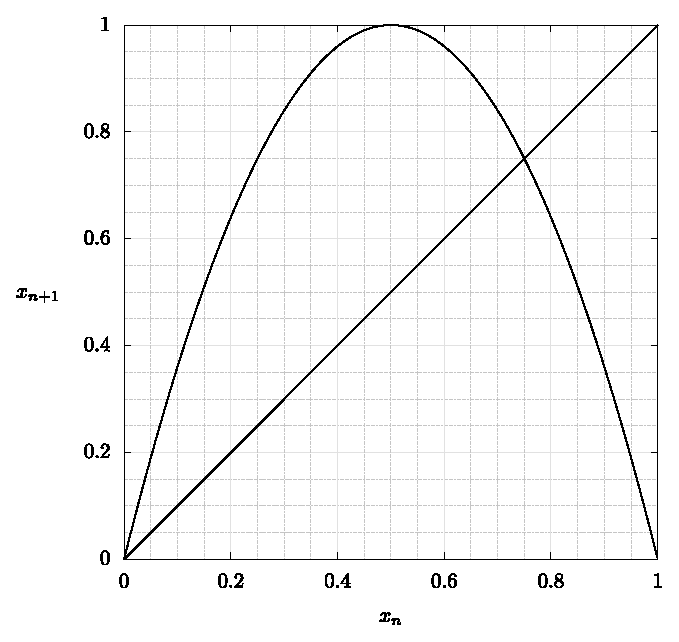
\includegraphics[width=0.6\textwidth]{F1_logistic_curve}
            \label{fig:F1_logistic_curve}
        \end{figure}

        En la Figura \ref{fig:F0_mapdiagram} también se muestra una recta descrita por $x_{n+1} = x_{n}$, a $45^{\circ}$ cuyas intersecciones con la parábola dan los valores de $x$ que no cambian con el tiempo. Para un mapa cuadrático, hay dos intersecciones de este tipo, que corresponden a las soluciones de la ecuación cuadrática que resultan de establecer $x_{n+1} = x_{n} = x^{*}$. Las soluciones $x^{*} = 0$ y $x^{*} = 1 - 1/A$ son llamados puntos fijos del mapa.

        \subsection{Diagrama de cobwebs}

            Es interesante examinar cómo $x$ se aproxima a un punto fijo partiendo de una condición inicial $x_{o} \neq x^{*}$, esto lo hacemos con un diagrama de cobwebs. La Figura \ref{fig:F2_cobwebs_simple} muestra el diagrama de cobwebs del mapa logístico para $A = 2.8$. Los diagramas de cobwebs son una herramienta valiosa que nos permiten observar el comportamiento global de un sistema de manera intuitiva, proporcionando información complementaria a la obtenida mediante el análisis lineal. Son especialmente útiles resultan cuando el análisis lineal no es suficiente.

            Para construir el diagrama de cobwebs de un mapa iterado realizamos los siguientes pasos:

            Dado $x_{n+1} = f(x_{n})$ y una condición inicial $x_{0}$, trazar una línea vertical hasta que intersecte la gráfica $f$, esa altura es la salida $x_{1}$, en otras palabras dibujar una línea vertical desde $(x_{0}, 0) $ hasta $(x_{0}, x_{1})$. Después trazar una horizontal hasta intersectar con la linea diagonal $x_{n+1} = x_{n}$, es decir, dibujar una línea desde  $(x_{0}, x_{1}) $ hasta $(x_{1}, x_{1})$. Después trazar otra línea vertical hasta que intersecte la gráfica $f$ otra vez, una línea desde $(x_{1}, x_{1}) $ hasta $(x_{1}, x_{2})$. Repetir este proceso $n$ veces para generar los primeros $n$ puntos en la órbita.

            \begin{figure}[hbtp]
                \caption{Diagrama de cobwebs de mapa logístico con $A = 2.8$ y $x_{0} = 0.2$.}
                \centering
                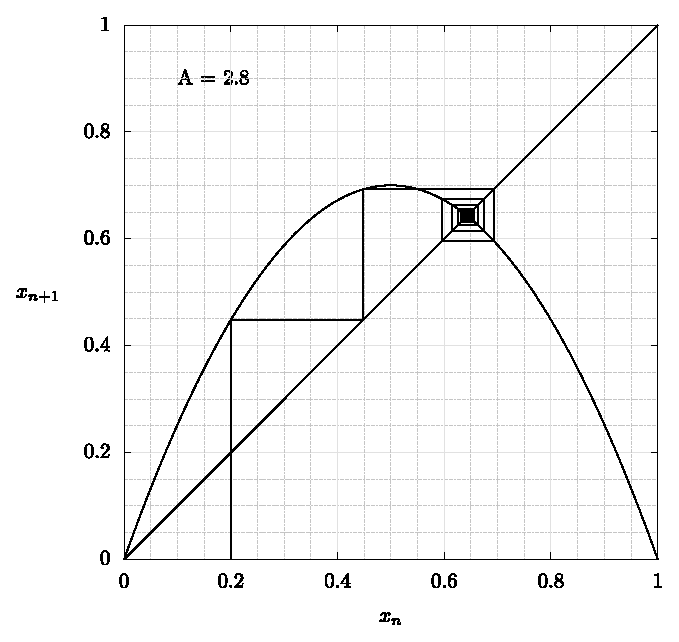
\includegraphics[width=0.6\textwidth]{F2_cobwebs_simple}
                \label{fig:F2_cobwebs_simple}
            \end{figure}

            Para el mapa logístico con $1 < A < 3,$ todos los puntos inicales en el intervalo $0 < x_{0} < 1$ se aproximan al punto fijo $x^{*} = 1 - 1/ A $, aunque la solución puede oscilar a su alrededor antes de llegar al valor final. El comportamiento recuerda al de un péndulo simple que oscila alrededor de la vertical antes de que la fricción lo lleve a reposar en su posición final. Otra manera de visualizar este comportamiento es gráfica la serie de tiempo, $x_{n}$ contra $n$, como se ve en la Figura \ref{fig:F3_time_series}. Es importante hacer la aclaración que se dibujaron lineas entre cada iteración para una mejor visualización, pero los datos son discretos. 

            \begin{figure}[hbtp]
                \caption{Serie de tiempo de mapa logístico con $A = 2.8$.}
                \centering
                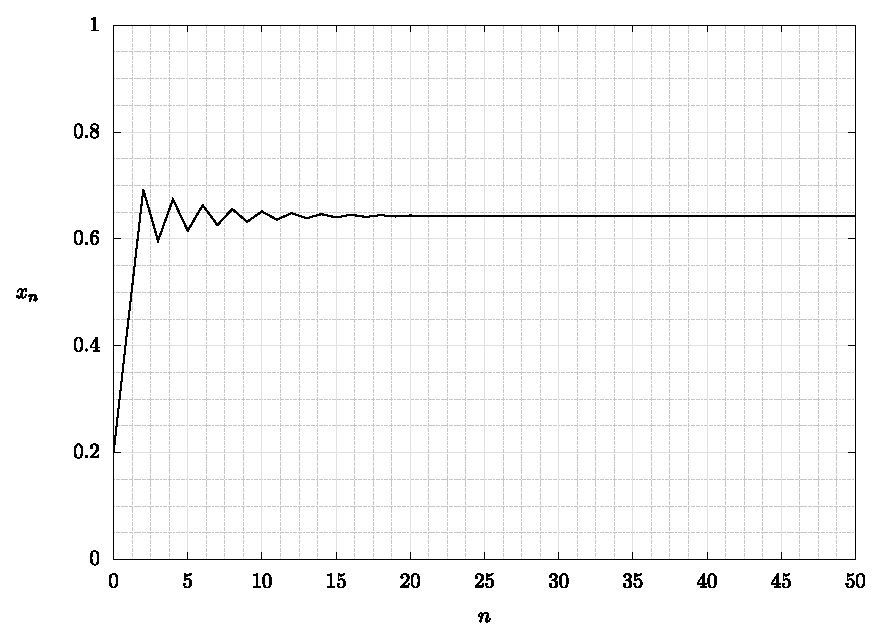
\includegraphics[width=0.6\textwidth]{F3_time_series}
                \label{fig:F3_time_series}
            \end{figure}

        \subsection{Análisis cualitativo del mapa logístico }

            En la ecuación de crecimiento exponencial en tiempo discreto (\ref{eq:crecimiento_exponencial}) cuando $A = \pm 1$ el comportamiento cambia abruptamente de acotado a no acotado. La ecuación logística se comporta de manera simular, excepto que hay más bifurcaciones y el comportamiento en varias regiones es más diverso e interesante. Es útil estudiar las bifurcaciones del mapa logístico debido a que las características generales son comunes a muchos sistemas caóticos. Consideraremos sólo valores positivos de $A$ y $x$.

            \begin{itemize}
                \item Caso $0 < A < 1$

                    En este rango la parábola solo puede intersectar a la linea de $45^{\circ}$ una vez en valores no negativos, y por lo tanto solo hay un punto fijo en $x^{*} = 0$. Todas las condiciones iniciales en el rango $0 < x_{o} < 1$ son atraídos hacia el punto $x^{*} = 0$. Decimos que estos puntos se encuentran dentro de una cuenca de atracción de $x_{0}$ y que el punto fijo $x_{0}$ es estable. Todos los puntos dentro de la cuenca de atracción se acercan al punto fijo con cada iteración. La no linealidad tiene poco efecto después de las primeras iteraciones. Los valores de $x_{0}$ fuera de de la cuenca de atracción están no acotados, escapan al infinito.

                \item Caso $1 < A < 3$

                    Al igual que con la ecuación (\ref{eq:crecimiento_exponencial}), para A = 1 se produce una bifurcación y el punto fijo en $x^{*} = 0$ se vuelve inestable. El atractor se convierte en un repulsor. Si $x$ resulta ser exactamente cero, permanecerá así, pero si es incluso ligeramente positivo, crecerá inicialmente a un ritmo exponencial. La situación es como la de un lápiz apoyado sobre su extremo puntiagudo. El más mínimo empujón hará que se caiga. Sin embargo, a diferencia de la ecuación (\ref{eq:crecimiento_exponencial}) en la que las soluciones son ilimitadas, el mapa logístico en $A = 1 $ desarrolla un nuevo punto fijo en $x^{*} = 1- 1/A = 0$ que se aleja de cero para $A > 1$. Si $A$ no es demasiado grande, entonces ese punto es un atractor porque todos los valores iniciales en el rango $0 < x_{0} < 1$ son atraídos hacia él y finalmente se asientan en él. Decimos que el estado final es un ciclo de periodo 1, o simplemente un ciclo de 1, porque cada iteración es la misma que la anterior. Si la ecuación logística estuviera modelando la población de bacterias, entonces predeciría un crecimiento exponencial inicial para este rango de $A$, pero un estado estacionario final en el que el número de bacterias no cambia.

                \item Caso $3 < A < 3.44948\ldots$

                    Para $A = 3$, el punto fijo en $x^{*} = 1 - 1/A$ sigue existiendo, pero cambia de estable a inestable, convirtiéndose en un repulsor. Esta bifurcación se produce cuando la pendiente de la parábola en el punto fijo es igual a $-1$. Para $A > 3$ tenemos un crecimiento exponencial alejándonos del punto, en lugar de una caída exponencial hacia él. Como la pendiente es negativa, la solución oscila a ambos lados del punto fijo mientras se aleja, igual que en la ecuación (\ref{eq:crecimiento_exponencial}) con $ A < -1$. De ahí que la bifurcación en $A = 3$ se denomine flip. Sin embargo, el crecimiento no continúa para siempre. En su lugar, se acerca a una condición en la que cada iteración es la misma $x_{n} = x_{n+2} = x_{n+4}$ como se muestra en el diagrama de cobwebs de la Figura \ref{fig:F5_cobwebs_bifurcation}. 

                    \begin{figure}[hbtp]
                        \caption{Diagrama de cobwebs de mapa logístico con $A = 3.2$ y $x_{0} = 0.1$.}
                        \centering
                        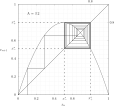
\includegraphics[width=0.6\textwidth]{F5_cobwebs_bifurcation}
                        \label{fig:F5_cobwebs_bifurcation}
                    \end{figure}

                    Con un poco de álgebra, esta condición puede reducirse a una ecuación de cuarto grado

                    \begin{equation}
                        A^{3} x^{4} - 2 A^{3} x^{3} + A^{2} (A + 1) x^{2} - (A^{2} -1)x = 0
                        \label{eq:cuarto_orden}
                    \end{equation}

                    Como cualquier ecuación de cuarto orden, tiene cuatro raíces. Una es $x^{*} = 0$, otra es $x^{*} = 1 - 1/A$. La factorización de estos términos reduce la ecuación (\ref{eq:cuarto_orden}) a una ecuación cuadrática

                    \begin{equation}
                        A^{2} x^{2} - A (A + 1) x + A + 1 = 0
                        \label{eq:segundo_orden}
                    \end{equation}
                    cuyas raíces son

                    \begin{equation}
                        x_{\pm}^{*} = \frac{A + 1 \pm \sqrt{(A-3) (A + 1)} }{2A} 
                        \label{eq:raices}
                    \end{equation}

                    Para $-1 < A < 3$, la cantidad dentro de la raíz cuadrada es negativa, y no existe una solución real. Para $A > 3$ hay dos raíces reales entre las cuales $x$ oscila en iteraciones sucesivas en el estado estacionario. Este es un ejemplo de un ciclo de 2. Se trata de un atractor cíclico o periódico ya que casi cualquier condición inicial en el intervalo unidad se aproxima a él. En tal caso, las bacterias abundarían una hora, escasearían a la siguiente y volverían a abundar. Obsérvese que para $A = 3$, la ecuación (\ref{eq:raices}) tiene una única raíz en $x^{*} = 2/3$, que es lo mismo que $x^{*} = 1 - 1/A$, lo que significa que el ciclo de 2 bifurca continuamente. 

                \item Caso $3.44948\ldots < A < 3.56994\ldots$

                    El ciclo de 2 existe para todo $A > 3$, pero se vuelve inestable cuando $A$ alcanza un valor en el que la pendiente del mapa de segunda iteración evaluado en $x = x^{*}$ según la ecuación (\ref{eq:cuarto_orden}) es igual a $-1$. El cálculo conduce a una ecuación cuadrática

                    \begin{equation}
                        A^{2} - 2A - 5 = 0      
                    \end{equation}
                    cuya raíz positiva es $A = 1 + \sqrt{6} = 3.449490\ldots$. En esta bifurcación, el ciclo de 2 se vuelve inestable, y nace un ciclo de 4 estable. El mapa logístico puede tener como máximo una órbita periódica estable para cada valor de $A$. Sin embargo, esta propiedad no la comparten todos los mapas unimodales unidimensionales. 

                    El proceso continúa con sucesivas duplicaciones de periodos (en cascada), apareciendo un nuevo periodo justo cuando el anterior se vuelve inestable. El inicio de estos desdoblamientos es cada vez más difícil de calcular, tanto analíticamente como numéricamente. Los próximos desdoblamientos se muestran en la Tabla \ref{tab:periodos}.

                    \begin{table}[htbp]
                        \caption{Diferentes número de ciclos para diferentes valores de $A$.}
                        \begin{center}
                            %\resizebox{0.8\linewidth}{!}{ 
                            \begin{NiceTabular}{|l|l|}
                                \CodeBefore
                                \rowcolor{lightgray}{1}
                                \Body
                                \hline
                                \textbf{Valores de A}  & \textbf{Número de ciclos}\\
                                \hline
                                $A_{1} = 3.000000\ldots$ & 2\\
                                \hline
                                $A_{2} = 3.449490\ldots$ & 4\\
                                \hline
                                $A_{3} = 3.544090\ldots$ & 8\\
                                \hline
                                $A_{4} = 3.564407\ldots$ & 16\\
                                \hline
                                $A_{5 } = 3.568759 \ldots$ & 32  \\
                                \hline
                                $A_{6 } = 3.569692 \ldots$ & 64  \\
                                \hline
                                $A_{7 } = 3.569891 \ldots$ & 128 \\
                                \hline
                                $A_{8 } = 3.569934 \ldots$ & 256 \\
                                \hline
                                $A_{9 } = 3.569943 \ldots$ & 521 \\
                                \hline
                                $A_{10} = 3.569945 \ldots$ & 1024\\
                                \hline
                                $\ldots \ldots \ldots \ldots \ldots \ldots$ & $\ldots \ldots$ \\
                                \hline
                                $A_{\infty}  = 3.5699456718 \ldots$ & punto de acumulación\\
                                \hline
                            \end{NiceTabular}
                            %}
                        \label{tab:periodos}
                        \end{center}
                    \end{table}

                    Las duplicaciones del periodo se acercan sucesivamente y acaban acumulándose en el punto $A_{\infty}  = 3.5699456718 \ldots$ conocido como punto de acumulación. En este punto, el periodo se hace infinito (nunca se repite), y la órbita visita infinitos valores de $x$ pero llena una porción insignificante del intervalo interior unitario $(0 < x < 1)$. El espacio entre bifurcaciones sucesivas se aproxima a una constante

                    \begin{equation}
                        \delta = \lim_{n \to \infty} \frac{A_{n} - A_{n-1} }{ A_{n+1} - A_{n} }  = 4.669201 \ldots
                    \end{equation}
                    conocida como el número de Feigenbaum. Las bifurcaciones vienen dadas aproximadamente por $A_{k} \approx A_{\infty} - 1.542 \delta^{-k}$. Una propiedad importante de la constante $\delta$ es su universalidad, ya que tiene el mismo valor para todos los mapas unimodales con un máximo cuadrático. Se trata de una nueva contante matemática, tan básica para la duplicación de periodos $\pi$ para los círculos. La duplicación del periodo con aparentemente la misma constante se ha observado en muchos experimentos, incluyendo fluidos turbulentos, circuitos electrónicos, láseres, reacciones químicas, grifos que gotean, instrumentos musicales, e incluso sistemas biológicos que no se describen obviamente mediante mapas unidimensionales, como los latidos del corazón.

                \item Caso $ 3.56994 < A < 4$

                    Cuando $A$ aumenta más allá del punto de acumulación, se desencadena el caos. El período es infinitamente largo y regiones finitas del intervalo unitario son visitadas por la órbita. Sin embargo, existen infinitas ventanas (rangos de $A$) de periodicidad. Todos los periodos están representados, pero la anchura de la ventana disminuye a medida que aumenta el periodo. Cada ventana de periodicidad aparece abruptamente a medida que $A$ aumenta y contiene su propia ruta de duplicación de periodos de vuelta al caos con el mismo número de Feigenbaum. Por ejemplo, la ventana prominente de período 3 comienza en $A = 1 + = 3.82842712\ldots$, aunque la demostración es difícil. La órbita de período 3 es especial, porque Sarkovskii y más tarde Li y Yorke (1975) demostraron independientemente que un mapa continuo unidimensional con una órbita de período 3 para un valor de parámetro particular tiene órbitas de todos los períodos (incluido el infinito) para ese parámetro y, por lo tanto, será caótico si todas esas órbitas son inestables. Lo contrario no es cierto, los sistemas caóticos no necesitan tener una órbita de período 3. Cada período superior a 3 ocurre más de una vez. Por ejemplo, hay dos ventanas de período 4, tres ventanas de período 5, cinco ventanas de período 6, etc. Todo el comportamiento puede resumirse en un diagrama de bifurcación como el de la Figura \ref{fig:F4_bifurcation}. Este diagrama representa todos los valores posibles de $x$ en el estado final después de que los transitorios iniciales hayan desaparecido en función del parámetro de control $A$. Los puntos de bifurcación, son evidentes.

                    \begin{figure}[hbtp]
                        \caption{Diagrama de bifurcación de mapa logístico.}
                        \centering
                        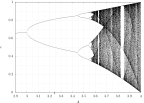
\includegraphics[width=0.6\textwidth]{F4_bifurcation}
                        \label{fig:F4_bifurcation}
                    \end{figure}

                \item Caso $A = 4$

                    El caso $A = 4$ es especial porque vuelve a mapear el intervalo unitario sobre sí mismo. Un mapa con esta propiedad se llama endomorfismo. Se puede imaginar el eje $x$ entre cero y uno como una banda elástica, que con cada iteración se estira de modo que su punto medio, $x_{n} = 0.5$, alcanza $x_{n+1} = 1$ y luego el extremo lejano $x_{n} = 1$ se pliega de vuelta hacia $x_{n+1} = 0$. El estiramiento y plegamiento son responsables del caos. Dos condiciones iniciales cercanas se separan debido al estiramiento, mientras que el plegamiento las mantiene acotadas. El estiramiento no es uniforme, sin embargo, debido a que es largo (un factor de cuatro por iteración) en $x = 0$ y $x=1$ pero infinitamente negativo en $x = 0.5$. En promedio el estiramiento es un factor de dos, como sugiere el hecho que se mapea de sobre sí mismo dos veces.

                    La iteración $x_{n}$ tiene dos preimagenes $x_{n-1}$ dadas por

                    \begin{equation}
                        x_{n-1} = 0.5 \pm \sqrt{0.25 - x_{n}/A} 
                    \end{equation}
                    que no suelen coincidir. En consecuencia, en cada iteración se pierde un bit de información (un factor de 2) ya que no hay forma de saber de qué preimagen procede cada valor (decimos que el mapa es no invertible, siendo en este caso de dos a uno), en contraste con un mapa invertible (de uno a uno) en el que existe una preimagen única. Esta pérdida exponencial de información equivale al crecimiento exponencial de los errores en la condición inicial que caracteriza al caos. La no invertibilidad es necesaria para el caos en los mapas unidimensionales, pero no para los mapas en dimensiones superiores. El caos se puede mostrar en un diagrama de cobwebs, como en la Figura \ref{fig:F7_cobwebs}, o directamente en un gráfico de iteraciones sucesivas o serie de tiempo, como en la Figura \ref{fig:F8_time_series}.

                    \begin{figure}[hbtp]
                        \caption{Diagrama de cobwebs de mapa logístico con $A = 4.0$ y $x_{0} = 0.1$.}
                        \centering
                        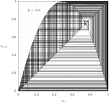
\includegraphics[width=0.6\textwidth]{F7_cobwebs}
                        \label{fig:F7_cobwebs}
                    \end{figure}

                    \begin{figure}[hbtp]
                        \caption{Serie de tiempo de mapa logístico con $A = 4.0$.}
                        \centering
                        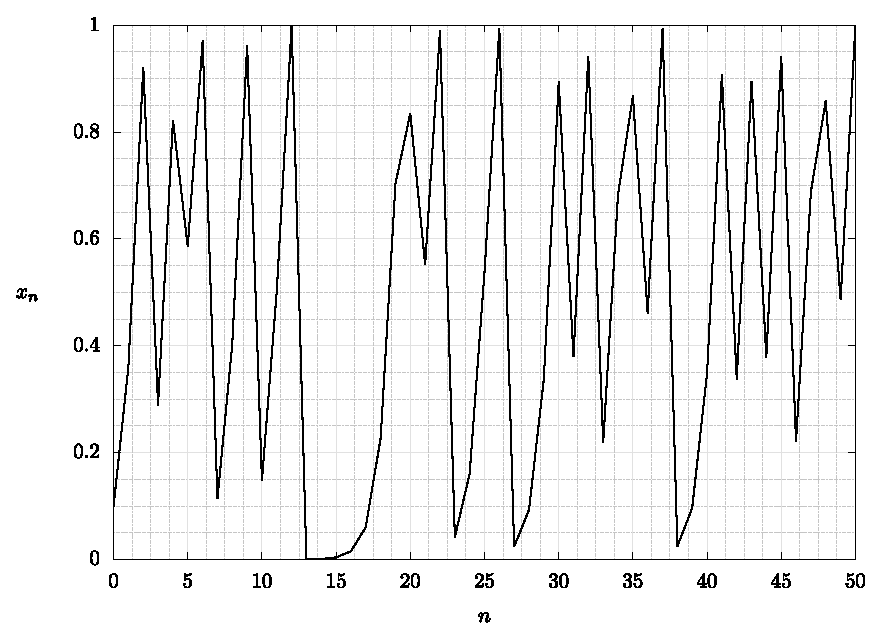
\includegraphics[width=0.6\textwidth]{F8_time_series}
                        \label{fig:F8_time_series}
                    \end{figure}

                    Aunque el comportamiento parece aleatorio, un examen más detallado revela el crecimiento exponencial en valores pequeños de $x_{n}$, valores pequeños de $x_{n}$ que siguen a uno grande y una oscilación creciente alrededor del punto fijo inestable en $x_{n} = 1 — 1/A = 0.75$. Es sorprendente que una simple ecuación cuadrática pueda exhibir un comportamiento tan complejo. Si la ecuación logística con $A = 4$ modelara el crecimiento de bacterias, entonces su población exhibiría fluctuaciones erráticas. El mapa logístico con $A = 4$, a veces llamado mapa de Ulam y escrito en la forma equivalente $x_{n+1} = 1 - 2 x_{n}^{2}$, fue estudiado por Ulam mucho antes de la era del caos moderno. Ulam y von Neumann lo propusieron como un generador de números aleatorios por computadora en 1947.

                    El mapa logístico con $ A = 4 $ es especial en muchos sentidos. Es totalmente caótico en el sentido de que casi todos los puntos del intervalo unitario son eventualmente visitados por cualquier condición inicial, una propiedad conocida como transitividad topológica. Este hecho y la simplicidad de la ecuación nos permite calcular varias propiedades especiales del mapa logístico con $ A = 4 $.

                \item Caso $A > 4$

                    Para $A > 4$, el pico de la parábola es superior a uno. Por lo tanto, la mayoría de las condiciones iniciales tienen iteraciones que eventualmente alcanzan $x_{n} > 1$. Cuando esto ocurre, la siguiente iteración es negativa, y el repulsor en $x = 0$ empuja la órbita rápidamente a menos infinito. Así, la mayoría de las órbitas son ilimitadas para $A > 4$. Sin embargo, el punto fijo inestable en $x^{*} = 1 - 1/A$ persiste para $A > 4$, al igual que todas las órbitas periódicas inestables, como el ciclo 2 dado por la ecuación (\ref{eq:raices}). La órbita de período 2 oscila entre un valor ligeramente superior a cero y un valor incluso ligeramente inferior a uno. 

        \end{itemize}

    \newpage
        \subsection{Análisis teórico del mapa logístico}

            Consideremos la ecuación $x_{n+1} = A x_{n} (1 - x_{n})$ para $0 \leq x_{n} \leq 1$ y $0 \leq A \leq 4$. Los puntos fijos satisfacen $x^{*} = f(x^{*}) = A x^{*}(1 - x^{*})$. Por lo tanto $x^{*} = 0$  o $x^{*} = 1 - 1/A$. El origen es un punto fijo para todas las $A$, mientras que $x^{*} = 1 - 1/A$ solo es valido para las $x \geq 1$. La estabilidad depende de $f'(x^{*}) = A - 2Ax^{*}$. Como $f'(0) = A $ el origen es estable para $A < 1$ e inestable para $A > 1$. En el otro punto fijo, $f'(x^{*}) = A - 2 A \left( 1 - 1/A \right) = 2 - A$. Entonces $x^{*} = 1 - 1/A$ es estable para $1 < A < 3$ e inestable para $A > 3$.

            En la Figura \ref{fig:F6_many_logistic_curve} se muestra un análisis gráfico de cómo se comporta el mapa logístico para distintos valores de $A$. Para $A < 1$ la parábola está por debajo de la diagonal, y el origen es el único punto fijo. A medida que $A$ aumenta, la parábola se hace más alta, haciéndose tangente a la diagonal en $A = 1$. Para $A > 1$ la parábola intersecta la diagonal en un segundo punto $x^{*} = 1 - 1/A$, mientras que el origen pierde estabilidad. Así vemos como $x^{*}$ se bifurca desde el origen en una bifurcación transcrítica en $A = 1$. 

            \begin{figure}[hbtp]
                \caption{Gráfica de mapa logístico para distintos valores de $A$.}
                \centering
                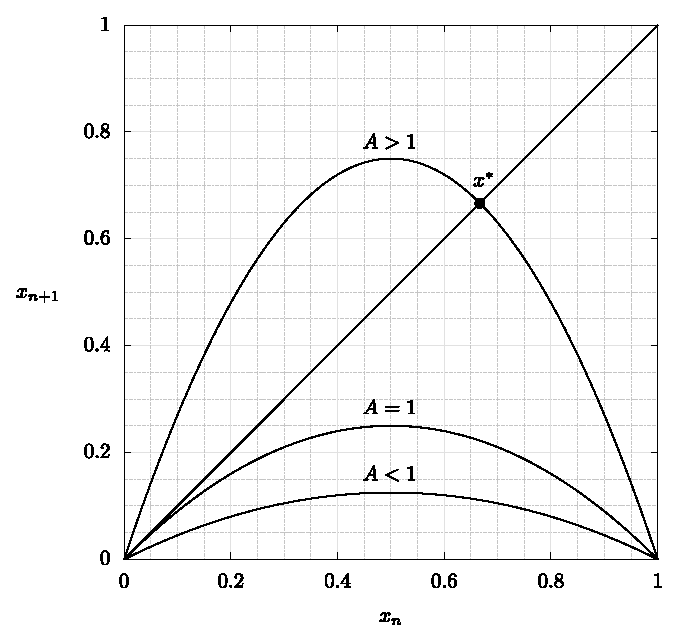
\includegraphics[width=0.6\textwidth]{F6_many_logistic_curve}
                \label{fig:F6_many_logistic_curve}
            \end{figure}
            
            Cuanto más crece $A$, más allá de 1, la pendiente en $x^{*}$ se vuelve cada vez más empinada, y $x^{*}$ pierde estabilidad. La pendiente crítica ocurre cuando $f'(x^{*}) = -1$, la cual se obtiene cuando $A = 3$. La bifurcación resultante se denomina bifurcación flip.

            Las bifurcaciones flip se asocian a menudo con la duplicación del período. En el mapa logístico, la bifurcación en $A = 3$ da lugar a un ciclo 2. Un ciclo 2 existe si y sólo si hay dos puntos $p$ y $q$ tales que $f(p) = q$  y $f(q) = p$. Equivalentemente, $p$ debe satisfacer que $f(f(p)) = p$, donde $f(x) = Ax (1 - x)$. Por tanto, $p$ es un punto fijo del \emph{mapa de segunda iteración}. Como $f(x)$ es un polinomio de segundo grado, $f(f(x))$ es un polinomio de cuarto grado.

            Para encontrar $p$ y $q$, necesitamos resolver los puntos en los que la gráfica intersecta la diagonal, es decir, necesitamos resolver la ecuación de cuarto grado $f(f(x)) = x$. Los puntos $x^{*} = 0$ y $x^{*} = 1 - 1/A$ son soluciones triviales de la ecuación. Si factorizamos estos puntos fijos, el problema se reduce a resolver una ecuación cuadrática. 

            La expansión de la ecuación $f(f(x)) -x = 0$ da $A^{2}x(1-x) [1 - Ax(1-x)] -x = 0$. Después de factorizar $x$ y $x - (1-1/A)$ por división larga, y resolver la ecuación cuadrática resultante, obtenemos un par de raíces:

            \begin{equation}
                p,q = \frac{A + 1 \pm \sqrt{(A-3) (A+1)} }{2A} 
            \end{equation}
            que son reales para $A > 3$. Por lo tanto, existe un ciclo doble para todo $ A > 3 $. En $ A = 3 $, las raíces coinciden y son iguales a $x^{*} = 1 - 1/A = 2/3$, lo que demuestra que el ciclo 2 bifurca continuamente a partir de $x^{*}$. Para $A < 3$ las raíces son complejas, lo que significa que no existe un ciclo 2.

             Para realizar el análisis de estabilidad es necesario seguir la siguiente estrategia. Para analizar la estabilidad de un ciclo, se reduce el problema a una pregunta sobre la estabilidad de un punto fijo de la siguiente manera. Tanto $p$ y $q$ son soluciones de $f(f(x)) = x$, por lo tanto $p$ y $q$ son puntos fijos del mapa de segunda iteración $f(f(x))$. El ciclo 2 original es estable precisamente si $p$ y $q$ son puntos fijos estables para $f(f(x))$.

            Ahora que el problema se reduce a analizar la estabilidad de los puntos fijos de otro mapa. Para determinar si $p$ es un punto fijo estable de $f(f(x))$, calculamos el multiplicador:

            \begin{equation}
                \lambda = \frac{d}{dx} ( f( f(x) ) )_{x=p} = f'(f(p))f'(p) = f'(q)f'(p)
            \end{equation}

            Se obtiene la misma $\lambda$ para $x = q$ por simetría. Por lo tanto, cuando las ramas $p$ y $q$ se bifurcan, deben hacerlo simultáneamente. Después de realizar las derivadas y realizar las evaluaciones $p$ y $q$, obtenemos:

            \begin{eqnarray}
                \lambda & = & A(1-2q) A(1-2p)\\
                    & = & A^{2} [1 - 2(p+q) + 4 pq]\\
                    & = & A^{2} [1 - 2 (A+1)/A + 4(A+1)/A^{2}] \\
                    & = & 4 + 2 A - A^{2}
            \end{eqnarray}

            Por lo tanto el ciclo 2 es linealmente estable para $|4 + 2A + A^{2}| < 1$ entonces $3 < A < 1 + \sqrt{6}$. Los métodos analíticos para las próximas bifurcaciones se vuelven poco manejables. Se pueden obtener otros resultados exactos pero son difíciles de conseguir. 

